\documentclass[../pbr.tex]{subfile}

\begin{document}
\section{Ray Marching}%
\label{sec:ray_marching}

After the ray has been case from the observer, then next step is to determine
what object it hits in the scene, if any. This process is the core the any path
tracer or ray tracer.

In most ray tracing or path tracing systems, the preferred implementation is to
use a ray tracer. The method that Specula uses is build off of the basis of a
ray tracer, so we will explain that first.

For these explanations we will consider a scene with three circles and a plane.
This example scene is shown in Figure \ref{fig:p1_2d_scene}.

\begin{figure}[htpb]
\begin{center}
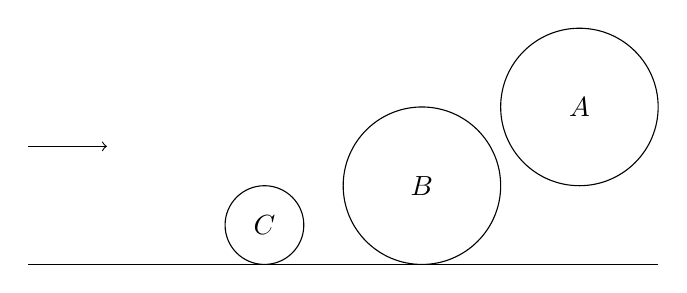
\begin{tikzpicture}[scale=1, transform shape]
  \draw (-3.0,0.0) -- (5.0,0.0);
  \draw (4.0, 2.0) circle (1.0) node {$A$};
  \draw (2.0, 1.0) circle (1.0) node {$B$};
  \draw (0.0, 0.5) circle (0.5) node {$C$};
  \draw[->] (-3.0,1.5) -- (-2.0,1.5);
\end{tikzpicture}
\end{center}
\caption{Sample scene for explanation}%
\label{fig:p1_2d_scene}
\end{figure}

\subsection{Ray Tracing}%
\label{sub:ray_tracing}

Ray tracing proceeds by calculating the rays intersection with all object in
the scene. For our example, the ray will intersect with circle $A$ and $B$. It
will actually intersect both of these twice. We will call these point $A_1$,
$A_2$, $B_1$, and $B_2$. Then by sorting these intersection points for which is
closest, we find where the intersection point is. This example is depicted in
Figure \ref{fig:p1_2d_scene2}, and we notice that the nearest intersection is
at point $B_1$, and we can continue processing from that point.

\begin{figure}[htpb]
\begin{center}
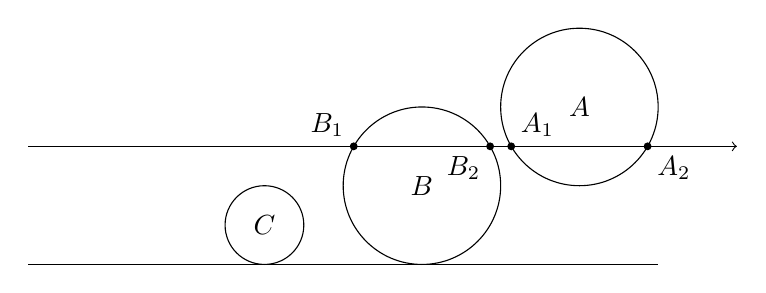
\begin{tikzpicture}[scale=1, transform shape]
  \draw (-3.0,0.0) -- (5.0,0.0);
  \draw (4.0, 2.0) circle (1.0) node {$A$};
  \draw (2.0, 1.0) circle (1.0) node {$B$};
  \draw (0.0, 0.5) circle (0.5) node {$C$};
  \draw[->] (-3.0,1.5) -- (6.0,1.5);
  \fill (1.1339,1.5) circle (0.05) node [above left] {$B_1$};
  \fill (2.8660,1.5) circle (0.05) node [below left] {$B_2$};
  \fill (3.1339,1.5) circle (0.05) node [above right] {$A_1$};
  \fill (4.8660,1.5) circle (0.05) node [below right] {$A_2$};
\end{tikzpicture}
\end{center}
\caption{Sample scene with ray tracing}%
\label{fig:p1_2d_scene2}
\end{figure}

To solve for these intersection points we first consider the spherical shell
as a collection of points. Thus we can rewrite the equation of a sphere as
\begin{align*}
   {\left(x-x_0\right)}^2+{\left(y+y_0\right)}^2+{\left(z+z_0\right)}^2&=r^2\\
   {\left\Vert P-C\right\Vert}^2&=r^2.
\end{align*}
Where $P$ is a point on the sphere, and $C$ is the center point of the sphere,
with radius $r$. We can also consider the equation for the ray as
\begin{align*}
   P(t)=A+tB,
\end{align*}
where $A$ is the origin of the ray, and $B$ is the direction that
the ray is traveling in, and $t$ is some scalar denoting the distance along the
ray in the direction of $B$. Combining these two equations we find
\begin{align*}
  {\left\Vert A+tB-C\right\Vert}^2&=r^2\\
  \text{dot}\left(A+tB-C,A+tB-C\right)&=r^2
\end{align*}
Expanding this we find
\begin{align*}
  \text{dot}\left(B,B\right)t^2+\text{dot}\left(B,A-C\right)2t+\text{dot}\left(A-C,A-C\right)-r^2=0.
\end{align*}
Using the quadratic formula we can solve for $t$, and find
\begin{align*}
   t=\frac{-2\text{dot}\left(B,A-C\right)\pm\sqrt{{4\text{dot}\left(B,A-C\right)}^2-4\text{dot}\left(B,B\right)\left(\text{dot}\left(A-C,A-C\right)-r^2\right)}}{2\text{dot}\left(B,B\right)}
\end{align*}
One we have calculated $t$, we can determine the point of intersection by
computing $A+tB$ with this calculated value for $t$. A similar process is done
for all other shapes in the scene, and then the smallest $t$ value is selected,
and that intersection point is used as for further computation.

\subsection{Ray Marching}%
\label{sub:ray_marching}

The method of ray marching is similar to that of ray tracing, but it never
computes the exact intersection point of the ray and an object. The premises of
ray marching is to determine how far a ray can travel with the certainty of not
intersecting and object. Then the ray moves that far and the process is
repeated. When the distance it travels in a step is less than some value, then
it is considered as an intersection.

\begin{figure}[htpb]
\begin{center}
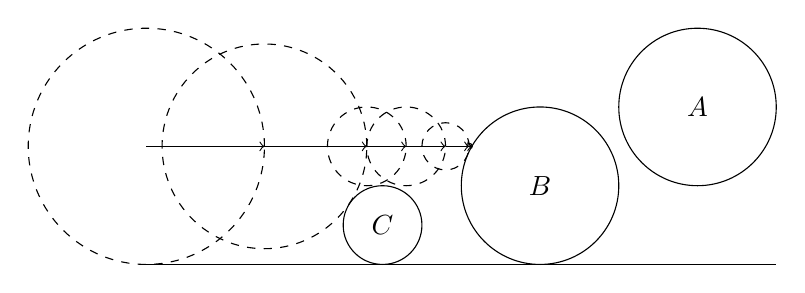
\begin{tikzpicture}[scale=1, transform shape]
  \draw (-3.0,0.0) -- (5.0,0.0);
  \draw (4.0, 2.0) circle (1.0) node {$A$};
  \draw (2.0, 1.0) circle (1.0) node {$B$};
  \draw (0.0, 0.5) circle (0.5) node {$C$};
  \draw[->] (-3.0,1.5) -- (-1.5,1.5);
  \draw[dashed] (-3.0,1.5) circle(1.5);
  \draw[->] (-1.5,1.5) -- (-0.2,1.5);
  \draw[dashed] (-1.5,1.5) circle(1.3);
  \draw[->] (-0.2,1.5) -- (0.3,1.5);
  \draw[dashed] (-0.2,1.5) circle(0.5);
  \draw[->] (0.3,1.5) -- (0.8,1.5);
  \draw[dashed] (0.3,1.5) circle(0.5);
  \draw[->] (0.8,1.5) -- (1.1,1.5);
  \draw[dashed] (0.8,1.5) circle(0.3);
  \draw[->] (1.1,1.5) -- (1.139,1.5);
  \draw[dashed] (1.1,1.5) circle(0.039);
\end{tikzpicture}
\end{center}
\caption{Sample scene with ray marching}%
\label{fig:p1_2d_scene3}
\end{figure}

This process is demonstrated in Figure \ref{fig:p1_2d_scene3}. Any any step, we
only need to compute the minimum distance to any object in the scene. This is
done recursively until the minimum distance is less than some value
$\varepsilon$.

These distance approximations are called distance functions. And ray marching
is the method that we will use for our renderer. The reasoning for this is that
it provides some features that other methods are unable to simulate. Although
it can be slower in the rendering process, if configured correctly it does not
cause any degradation to the resulting image.

\end{document}
